\chapter{Applications to graph theory}

\section{The Azuma-Hoeffding Inequality}

\begin{definition}
    A sequence $X_0, \ldots, X_n$ of random variables is consider a \textbf{martingale} if, for every $i \leq n$,
    \[ \E [X_{i+1} | X_i,\ldots, X_0] = X_i \] 
\end{definition}

A random graph $G = G(n)$ is a graph that has $n$ labeled vertices and produces an edge between 2 of them with a probability. Let $v_1, \ldots, v_n$ denote the vertices of $G$ and $e_1, \ldots, e_m$ all of the $\binom{n}{2}$ potential edges that $G$ can produce. Also, define each edge's indicator function as it follows,
\[\1_{e_k \in G} = \begin{cases}
    1, & e_k \in G\\
    0, & \mbox{otherwise} 
\end{cases} \] 
An edge exposure martingale is a sequence of random variables defined as the expected value of a function $f(G)$ which depends on the information of the first $j$ potential edges:

\[ X_j = \E [f(G) \;|\; \1_{e_1 \in G}, \ldots, \1_{e_j \in G}] \] 

Since all of the graph information is contained in its edges, the sequence transitions from no information: $X_0 = E(f(G))$, to the true value of the function: $X_m = f(G)$. Similarly, one can define a martingale which depends on how many vertices are revealed. The vertex exposure martingale is defined as it follows,

\[ X_i = \E [f(G) \;|\; \1_{\{v_k, v_j\}\in G}, \; k < j \leq i] \] 

The following inequality is to some extend an adapted version of Hoeffding inequality~\ref{hoeffding:bounded} for martingale random variables. If we stablish a limit for which a martingale varies from one step to another, the theorem then states that we can exponentially bound the tails of its distribution:

%% --- Azuma's inequality
\begin{theorem}[Azuma-Hoeffding inequality]\label{azuma}
    Let $X_0, \ldots, X_m$ be a martingale with $X_0 = 0$, and
    \[ |X_{i+1} - X_i| \leq 1, \hspace*{1em} \forall i < m. \]
    Then, for $t > 0$,
    \[ \P\{X_m > t\sqrt{m}\} < e^{-t^2 / 2}. \] 
\end{theorem}

\begin{proof}
    First, we must prove another inequality.
    \begin{lemma}
        Let $Y_1, \ldots, Y_m$ be random variables such that $|Y_i| \leq 1$ and $\E Y_i = 0$, and let $S_m = \sum_{i = 1}^m Y_i$. Then, for $\lambda > 0$,
        \[ \E[e^{\lambda Y_i}] \;\leq\; e^{\lambda^2 / 2}. \]
    \end{lemma}

    \begin{proof}

    \begin{tabular}{cc}
        \(\displaystyle h(x) = \frac{e^\lambda + e^{-\lambda}}{2} + \frac{e^\lambda - e^{-\lambda}}{2} \cdot x,  \)
        &\hspace*{2em}
        \begin{tabular}[c]{@{}l@{}}
        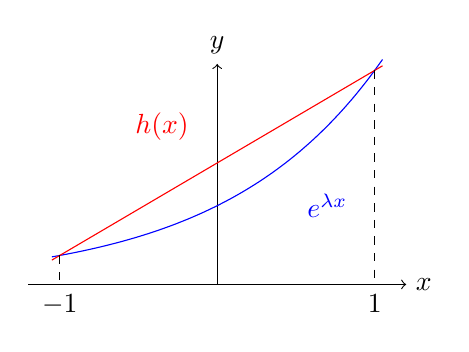
\begin{tikzpicture}
            \draw[->] (-2.4, 0) -- (2.4, 0) node[right] {$x$};
            \draw[->] (0, 0) -- (0, 2.8) node[above] {$y$};
            \draw[scale=1, domain=-2.1:2.1, smooth, variable=\x, blue] plot ({\x}, {e^(\x/2)});
            \draw[scale=1, domain=-2.1:2.1, smooth, variable=\y, red]  plot ({\y}, {(e+1/e)/2 + (e-1/e) * \y/4}); % Divided \x and \y by 2 on the 2nd coordinate to scale the y axis by 1/2.
                \node[text=red] at (-0.7,2) {$h(x)$};
            \node[text=blue] at (1.4,1) {$e^{\lambda x}$};
            \draw [dashed] (-2, {e^(-1)}) -- (-2,0)  node[below] {$-1$};
            \draw [dashed] (2, {e^(1)}) -- (2,0) node[below] {$1$};
        \end{tikzpicture} 
    \end{tabular}
    \end{tabular}

    As the picture above shows, $h(x)$ is the line that passes through the points $x = -1$ and $x = 1$ in the function $e^{\lambda x}$. Since $e^{\lambda x}$ is convex ($\lambda > 0$), it follows that $h(x) \geq e^{\lambda x} $ for $x \in [-1,1]$. Thus,

    \[\everymath{\displaystyle}\arraycolsep=1.8pt\def\arraystretch{1.8}
      \begin{array}{rcl}
        \E[e^{\lambda Y_i}] & \leq & \E[h(Y_i)] \\
        \text{\scriptsize ($h$ is linear)}& = & h(\E Y_i) = h(0)\\
        & = & \frac{e^\lambda + e^{-\lambda}}{2} = \cosh \lambda .
      \end{array}      
    \]
    Finally, $(2k)! \geq 2^k \cdot k! $, for every $k\in\N$. Thus,

    \[
        \E[e^{\lambda Y_i}]\leq \cosh \lambda \;=\; \sum_{k = 0}^\infty \frac{\lambda^{2k}}{(2k)!} \;\leq\; \sum_{k = 0}^\infty \frac{\lambda^{2k}}{2^k \cdot k!} \;=\; e^{\lambda^2 / 2}.
    \]

    \end{proof}

    Now, define $Y_i = X_i - X_{i-1}$. Then, by hypothesis, $|Y_i| \leq 1$ and
    \[ \E [Y_i | X_{i-1},\ldots, X_0] = \E [X_i - X_{i-1} | X_{i-1},\ldots, X_0] = X_i - X_i = 0. \] 
    Therefore, we can apply the previous inequality to assert,
    \[ \E [e^{\lambda Y_i} | X_{i-1},\ldots, X_0] \leq e^{\lambda^2/2}. \tag*{$ (\star) $}\]

    Using the formula $E[XY] = E_X [X E[Y|X]]$ we assert that
    \[ \E e^{\lambda X_m} \; = \;  \E\left[\prod_{i = 1}^{m-1} e^{\lambda Y_i} \cdot \E[e^{\lambda Y_m} | X_{m-1},\ldots, X_0]\right] \]

    We repeat this process $n$ times:
    \[ \everymath{\displaystyle}\arraycolsep=1.8pt\def\arraystretch{1.8}
        \begin{array}{r c c c l}
        & & \E e^{\lambda X_m}  =   \E \prod_{i = 1}^{m} e^{\lambda Y_i} \hfill\\
        & = & \E\left[\prod_{i = 1}^{m-1} e^{\lambda Y_i} \cdot \E[e^{\lambda Y_m} | X_{m-1},\ldots, X_0]\right] \hfill & \overset{(\star)}{\leq} & \E\left[\E \prod_{i = 1}^{m-1} e^{\lambda Y_i} \right] e^{\lambda^2 / 2}\\
        & = & \E\left[\prod_{i = 1}^{m-2} e^{\lambda Y_i} \cdot \E[e^{\lambda Y_{m-1}} | X_{m-2},\ldots, X_0]\right]e^{\lambda^2 / 2} & \overset{(\star)}{\leq} & \E\left[\E \prod_{i = 1}^{m-2} e^{\lambda Y_i} \right] e^{2\lambda^2 / 2}\\
        & = & \hfill\vdots\hfill & \leq & \hfill\vdots\hfill\\
        & = & \E\left[\E[e^{\lambda Y_{1}} |  X_0]\right]e^{\lambda^2 / 2} & \leq & \hfill e^{m\lambda^2/2} \hfill
    \end{array} \tag*{$ (*) $} \]
    At last, by setting $\lambda = t/\sqrt{m}$ we obtain,
    \[ \everymath{\displaystyle}\arraycolsep=1.8pt\def\arraystretch{1.8}
    \begin{array}{r c l}
        \P\{X_m > t\sqrt{m}\} & = & \P\{e^{\lambda X_m} > e^{\lambda t \sqrt{m}}\} \\
        \text{\scriptsize (Markov)}& \leq & \E[e^{\lambda X_m} ] e^{-\lambda t \sqrt{m}}\\
        & \overset{(*)}{\leq} & e^{m\lambda^2/2} \cdot e^{-\lambda t \sqrt{m}}\\
        \text{\scriptsize ($\lambda = t/\sqrt{m}$)} & = & e^{t^2/2} e^{-t^2} = e^{-t^2 / 2}.
    \end{array}    \tag*{$ (\bullet) $}
    \]
\end{proof}
%% --------------------

\begin{remark} We assumed that $X_0 = 0$ to lighten the notation. However, we can remove this restriction by replacing $X_m$ with $X_m - X_0$ in some crucial steps:
    \[\everymath{\displaystyle}\arraycolsep=1.8pt\def\arraystretch{1.8}
        \begin{array}{rl}
            & X_m-X_0 = \sum_{i = 1}^n Y_i\\
            \overset{(*)}{\implies} & \E e^{\lambda (X_m-X_0)} = \E \prod_{i = 1}^{m} e^{\lambda Y_i} \leq e^{m \lambda^2 / 2}\\
            \overset{(\bullet)}{\implies} & \P\{X_m-X_0 > t\sqrt{m}\} \leq e^{-t^2/2}
        \end{array} 
        \] 

\end{remark}    

In the following section we are going to present an application of the Azuma-Hoeffding inequality to prove the convergence to the mean of a fast (but not effective) approximation algorithm for the \textit{Travelling Salesman Problem}. 

\section{An Heuristic Algorithm for the Travelling Salesman Problem}

Let $X_1,\ldots, X_N$ be a sample of $N$ uniformly distributed points in a compact square $[0,L]\times [0,L]$. The algorithm divides this square in $M$ stripes of width $L/M$ each. Then, it connects each of the points in each of the stripes vertically and connects the top-most of one stripe with the top-most of the next one (or viceversa as the image below shows).

\begin{figure}[ht]\label{TSP:pic0}
    \centering
    \subfloat[Uniform sample]{\label{TSP:pic0.1}
        \includegraphics[width=0.33\textwidth]{../Simulation/TSPPictures/ex0.png}
    }
    \subfloat[Divide in $M$ stripes]{\label{TSP:pic0.2}
        \includegraphics[width=0.33\textwidth]{../Simulation/TSPPictures/ex1.png}
    }
    \subfloat[Join points vertically]{\label{TSP:pic0.3}
        \includegraphics[width=0.33\textwidth]{../Simulation/TSPPictures/ex2.png}
    }
\end{figure}

In the paper~\cite{gzyl1990physicist} the authors found that the optimal  number of stripes is $M^* = \floor{0.58 N^{1/2}}$. If $t_N$ is the TSP solution distance for our sample and $d_N$ is the algorithm's answer with the optimal $M^*$, then the error is asymptotically:
\[  \frac{d_N-t_N}{t_N} \approx 0.23.\] 

The result that we are going to show is that $d_n$ is very concentrated around its mean. In order to prove this, some modifications must be made to the algorithm's trajectory. Let $e_N$ be the distance of a new trajectory that satisfies the following conditions:
\begin{itemize}
    \item For any empty stripe in the plane we sum the length of its diagonal $\sqrt{L^2+ L^2/M^2}$ and then it skips the empty stripe.
    \item When there are no empty stripes, $e_N = d_N$ 
\end{itemize}
 Since the probability that any given stripe is empty converges exponentially to 0,
\[ \begin{array}{rl}
    {(1- 1/M)}^N & = {(1- 0.58^{-1} N^{-1/2})}^N\\[1em]
    & = {\left({(1- 1/M)}^{M}\right)}^{0.58^{-1} N^{1/2}}\\[1em]
    &  \sim \exp(-0.58^{-1} N^{1/2}).
\end{array} \] 


Let $\A_i := \sigma\{X_1,\ldots,X_i\}$ denote the sigma algebra corresponding to revealing the first $i$ points, $\A_0 = \{\emptyset, {[0,L]}^2\}$. The expected value of the trajectory $e_N$ given that we only know the positions of the first $i$ points in the sample is $\E (e_N | \A_i)$. Define
\[ Z_i = \E (e_N | \A_i) - \E (e_N | \A_{i-1}),  \]  
As the difference of this expectations when we reveal 1 more point. Note that since
\[ \E(Z_i | \A_i) =  \E (e_N | \A_i, \A_i) - \E (e_N | \A_{i-1}, A_i) = \E (e_N | \A_i) - \E (e_N | \A_i) = 0,\] 
$Z_1, \ldots, Z_N$ is the difference sequence of a vertex exposure martingale.

% \begin{figure}[ht]\label{TSP:pic1}
%     \subfloat[$i = 0$]{\label{TSP:pic1.1}
%         \includegraphics[width=0.25\textwidth]{../Simulation/TSPPictures/pic0.png}
%     }
%     \subfloat[$i = 1$]{\label{TSP:pic1.2}
%         \includegraphics[width=0.25\textwidth]{../Simulation/TSPPictures/pic1.png}
%     }
%     \subfloat[$i = 2$]{\label{TSP:pic1.3}
%         \includegraphics[width=0.25\textwidth]{../Simulation/TSPPictures/pic2.png}
%     }
%     \subfloat[$i = 4$]{\label{TSP:pic1.4}
%         \includegraphics[width=0.25\textwidth]{../Simulation/TSPPictures/pic3.png}
%     }

%     \subfloat[$i = 7$]{\label{TSP:pic1.5}
%         \includegraphics[width=0.25\textwidth]{../Simulation/TSPPictures/pic4.png}
%     }
%     \subfloat[$i = {12}$]{\label{TSP:pic1.6}
%         \includegraphics[width=0.25\textwidth]{../Simulation/TSPPictures/pic5.png}
%     }
%     \subfloat[$i = {18}$]{\label{TSP:pic1.7}
%         \includegraphics[width=0.25\textwidth]{../Simulation/TSPPictures/pic6.png}
%     }
%     \subfloat[$i = N = 50$]{\label{TSP:pic1.8}
%         \includegraphics[width=0.25\textwidth]{../Simulation/TSPPictures/ex2.png}
%     }
%     \caption{Evolution of the vertex exposure martingale}
% \end{figure}

Define $e_N^{[i]}$ as the distance of the trajectory when we remove the $i$-th point from the sample. Intuitively from the triangle inequality, we can obtain the following inequalities:
\[ e_N^{[i]} \leq e_N \leq e_N^{[i]} + 2 L/M, \]
meaning that revealing one point cannot increase more than 2 widths the distance of the trajectory. Thus,
\[ \|Z_i\|_\infty = \sup_{X_1,\ldots, X_N} \|\E (e_N | \A_i) - \E (e_N | \A_{i-1})\| \leq 2L/M. \tag*{$ (\star)$}.\]

On the other hand,
\[  e_N - \E e_N = \E (e_N | \A_N) - \E (e_N | \A_{0}) = \sum_{i = 1}^{N} Z_i.\]
Therefore, by the Azuma-Hoeffding inequality,
\[ \P \{ |e_N - \E e_N| > t \} \leq 2\exp\left(\frac{-t^2}{2}\sum_{i = 1}^{N} \|Z_i\|_{\infty}^2 \right). \] 
Finally,
\[ \sum_{i = 1}^{N} \|Z_i\|_{\infty}^2 \leq \frac{4NL^2}{M^2}, \]
which implies that
\[\P \{ |e_N - \E e_N| > t \} \leq 2\exp\left(\frac{-t^2}{2}\sum_{i = 1}^{N} \frac{4NL^2}{M^2} \right) \sim e^{-t^{2} K N}, \] 
for some $K\in \R^+$.

\section{Lipschitz Condition and Three Additional Examples}

Three examples from~\cite{alon2016probabilistic} will be exposed to illustrate some ideas that can be associated with the main inequality of this chapter. Furthermore, the usefulness of the Azuma-Hoeffding inequality in the study of graphs and metric spaces can be used in a more general frame by defining the Lipschitz condition.

\vspace*{1em}

Let $\Omega = A^B$ be the set of all functions $g: B\to A$ for which a probability measure is assigned
\[ \P\{g(b) = a\} = p(a,b),\hspace*{1em} \sum_{a\in A} p(a,b) = 1. \]
All the values $g(b)$ are mutually independent. Now, fix a chain of sets 
\[ \emptyset = B_0 \subset B_1 \subset \ldots \subset B_m = B,\hspace*{1em} \mathcal{B} = {\{B_i\}}_{i = 0}^m \]
and let $L: A^B \to \R$ be a functional. The martingale sequence $X_0,\ldots, X_m$ associated with $L$ and $\mathcal{B}$ is defined as it follows: For a fixed $h \in A^B$:

\[ X_i(h) = \E[ L(g) \;|\; g(b) = h(b),\; \forall b\in B_i ]. \] 

What this means is that, given that we know the values in $B_i$ of a function $h$, the martingale at the $i$-th step predicts the outcome of $L(h)$ based only on this information. The following definition and theorem have the purpose to make our lives easier when talking about the `boundness' of a martingale.

\begin{definition}
    A functional $L$ is said to satisfy the Lipschitz condition if for every $i < m$: Whenever two functions $g, g'$ differ only in $B_{i+1}- B_i$,
    \[ |L(g) - L(g')| \leq 1. \] 
\end{definition}

When we say that the outcome of $L$ won't change by more than 1 unit from one revelation to another, it means that it has the Lipschitz condition. The following theorem will connect this idea to Azuma's inequality:

\begin{theorem}\label{lipschitz-condition}
    The martingale associated with a functional $L$ with the Lipschitz condition satisfies:
    \[ |X_{i+1}(g)- X_i(g)| \leq 1,\hspace*{1em} \forall g\in A^B,\; \forall i < m. \] 
\end{theorem}

\begin{proof} The proof is adapted from~\cite{alon2016probabilistic} chapter 7. In the original proof, the author skips many steps that I believe are not trivial. Thus, I decided to restructure the proof using the same notation they used in the source material:

\subsubsection*{Preliminaries}
Our goal is to calculate $|X_{i+1}(h) - X_{i}(h)|$, so fix $h \in A^B$, $i\in \N$ and define

\[ p_{f}^{(j)} = \P\{g = f \;|\; g(b) = h(b),\; \forall b \in B_{j}\}.\; \forall j\in \N. \]

Now, $\forall j\in \N$, define $H^{(j)}\subset A^B$ to be the set of functions $f$ in which $h(b) = f(b)$ for every $b \in B_{j}$. In notation,

\[ H^{(j)} = \{f \in A^B: h(b) = f(b),\; \forall b \in B_j\}. \] 

Note that if $h' \not\in H^{(j)}$ and $g(b) = h(b)$ for every $b\in B_{j}$, then it would be imposible for $g$ to be equal to $h'$ because there would exist $b^* \in B_{j}$ such that $h'(b^*) \neq h(b^*) = g(b^*)$. Thus, if $h' \not\in H^{(j)}$, then $p_{h'}^{(j)} = 0$. This also implies that 
\[\sum_{h' \in H^{(j)}} p_{h'}^{(j)} = 1 \] 

\subsubsection*{Rewriting $X_{i+1}$}
From now on, $H$ without any index refers to $H^{(i+1)} =: H$
\[\everymath{\displaystyle}\arraycolsep=1.4pt\def\arraystretch{1.5}
    \begin{array}{rcl}
    X_{i+1}(h) & = & \E[ L(g) \;|\; g(b) = h(b),\; \forall b\in B_{i+1} ]. \\ 
    & = & \sum_{h' \in A^B} L(h') \cdot \P\{g = h' \;|\; g(b) = h(b),\; \forall b \in B_{i+1}\}\\
    & = & \sum_{h' \in H} L(h') \cdot p_{h'}^{(i+1)}
\end{array}\]


\subsubsection*{Rewriting $X_i$}
Like the previous step,
\[\everymath{\displaystyle}\arraycolsep=1.4pt\def\arraystretch{1.5}
    \begin{array}{rcl}
    X_{i}(h) & = & \sum_{f\in H^{(i)}} L(f) p_{f}^{(i)}
\end{array}\]
However, we want to write the sum of $X_{i}(h)$ in terms of $h' \in H$. Now, for $h' \in H$, let $H[h']$ be the set of $h^*$ such that $h^*, h'$ that can only differ in $B_{i+1}-B_{i}$. In notation,
\[ H[h'] = \left\{ h^*: \begin{matrix}
    h^*(b) = h'(b),\; \forall b\in B-B_{i+1}\\
    h^*(b) = h'(b) ,\; \forall b\in B_{i}
\end{matrix} \right\} \] 
Also, define for $h^* \in H[h']$
\[ q_{h^*} = \P\{g(b) = h^*(b),\; \forall b\in B_{i+1} \;|\; g(b) = h(b),\; \forall b\in B_{i} \}. \]
It follows from the definition of $H[h']$ and $H$ that
\[ \everymath{\displaystyle}\arraycolsep=1.4pt\def\arraystretch{1.5}
    \begin{array}{rcl}
    \sum_{h^* \in H[h']} q_{h^*} & = & \sum_{h^* \in H[h']} \P\left\{\begin{matrix} g(b) = h^*(b),\; \forall b\in B_{i+1}-B_i\\  g(b) = h^*(b) = h'(b) ,\; \forall b\in B_i \end{matrix} \;\Bigg|\; g(b) = h(b) = h'(b),\; \forall b\in B_{i} \right\} \\
     & = & \P\{g(b) = h'(b),\; \forall b\in B_{i} \;|\; g(b) = h'(b),\; \forall b\in B_{i} \}\\
     & = & 1.
\end{array} \]  

$\coprod$ is the notation I'm going to use for the disjoint union. Note that if $h_1'\neq h_2' \in H$, then both must differ in some $b \in B- B_{i+1}$. Thus, the following unions are disjoint
\[\everymath{\displaystyle}\arraycolsep=1.4pt\def\arraystretch{1.5}
    \begin{array}{rcl}
    \coprod_{h' \in H} H[h'] & = & 
    \coprod_{h' \in H} \left\{ h^*: \begin{matrix}
        h^*(b) = h'(b),\; \forall b\in B-B_{i+1}\\
        h^*(b) = h'(b) = h(b) ,\; \forall b\in B_{i}
    \end{matrix} \right\}\\
   \hfill\vdots\hfill & = & \coprod_{h' \in H} \left\{ h^*: \begin{matrix}
        h^*(b) = h'(b),\; \forall b\in B-B_{i+1}\\
        h^*(b) = h(b) ,\; \forall b\in B_{i}
    \end{matrix} \right\}\\
    \hfill\downarrow\hfill& = & \{h^*: h^*(b) = h(b) ,\; \forall b\in B_{i} \}\\
    \coprod_{h' \in H} \coprod_{h^* \in H[h']}\{h^*\} & = & H^{(i)}.
\end{array} \] 
Thus, we can make a partition of $X_i(h)$ iterating over $H$ and $H[h']$:
\[\everymath{\displaystyle}\arraycolsep=1.4pt\def\arraystretch{1.5} 
\begin{array}{lcl}
    \E[L(g) \;|\; g(b) = h(b),\; \forall b\in B_{i}] & = & \sum_{f\in H^{(i)}} L(f) p_{f}^{(i)}\\
    & = &  \sum_{h' \in H}\sum_{h^* \in H[h']} L(h^*) p^{(i)}_{h^*}
\end{array}\] 

Finally, for $h' \in H$ and $h^* \in H[h']$,
\[ \everymath{\displaystyle}\arraycolsep=1.4pt\def\arraystretch{1.5} 
\begin{array}{lll}
    & & p^{(i)}_{h^*} = \\
    & & \P\{g = h^* \;|\; g(b) = h(b),\; \forall b\in B_i\}\\
    & = & \P\{g = h^* | g(b) = h^*(b),\; \forall b\in B_{i+1} \} \cdot \P\{g(b) = h^*(b),\;\forall b\in B_{i+1} | g(b) = h^*(b),\; \forall b\in B_{i} \}\\
    & = & \P\{g = h' | g(b) = h(b),\; \forall b\in B_{i+1} \} \cdot q_{h^*}\\
    & = & p_{h'}^{(i+1)}\cdot q_{h^*}
\end{array}  \] 
\[ \implies X_i(h) = \sum_{h' \in H}\sum_{h^* \in H[h']} [L(h^*) q_{h^*}] \cdot p_{h'}^{(i+1)} \] 

\subsubsection*{Bound for $|X_{i+1}- X_i|$}
Combine the results from the two previous sections. For the second line, remember that $\sum_{h^*\in H[h']} q_{h^*} = 1$
\[ \everymath{\displaystyle}\arraycolsep=1.4pt\def\arraystretch{2.9} 
\begin{array}{rcl}
    |X_{i+1}(h)- X_i(h)| & = & \left|\sum_{h' \in H}p_{h'}^{(i+1)} \left[ L(h') - \sum_{h^* \in H[h']}  L(h^*)q_{h^*}\right] \right|\\
    & = & \left|\sum_{h' \in H}p_{h'}^{(i+1)} \sum_{h^* \in H[h']} q_{h^*}(L(h') - L(h^*)) \right|\\
    & \leq & \sum_{h' \in H}p_{h'}^{(i+1)} \sum_{h^* \in H[h']} q_{h^*} |L(h') - L(h^*)|
\end{array} \] 

By hypothesis, $|L(h') - L(h^*)| \leq 1$. Thus,

\[|X_{i+1}(h)- X_i(h)| \leq  \sum_{h' \in H}p_{h'}^{(i+1)} \sum_{h^* \in H[h']} q_{h^*} = \sum_{h' \in H}p_{h'}^{(i+1)} = 1. \] 

\end{proof}

With this theorem, we can talk with more freedom about the boundness of a martingale. The following three examples will illustrate some uses for Azuma's inequality in conjunction with the previous theorem.

\subsection*{Example 1}
Let $g \in {[n]}^{n}$ be a random vector (uniformly chosen) with $n$ entries, in which every entry is in $[n] = \{1,\ldots n\}$. Define $L(g)$ to be the amount of number that are not included in the vector,
\[ L(g) = \# \{ k \;:\; g_i \neq k,\; \forall i \in [n]\} = \sum_{k = 1}^{n} \1_{k \not\in g} \] 
For example,

\[ L(\underset{g_1}{1},\underset{g_2}{3},\underset{g_3}{1},\underset{g_4}{6},\underset{g_5}{4},\underset{g_6}{3}) = 2.\;\text{ (because 2 and 5 are missing)} \]

We can understand the process of choosing $g$ as independently assigning a random number in each of its coordinates. Thus, for a number $k \in \{1,\ldots, n\}$, the probability that this number is not in any of the entries of the vector is
\[\E \1_{k \not\in g} = \P\{g_i \neq k, \; \forall i\} = \prod_{i = 1}^n P\{g_i \neq k\} = {\left(1-\tfrac{1}{n}\right)}^n. \] 
Hence,
\[ \E L(g) = \sum_{k = 1}^n \P\{g_i \neq k, \; \forall i\} = n {\left(1-\tfrac{1}{n}\right)}^n \sim \frac{n}{e}. \] 
Now, define $B_i = \{1, \ldots, i\}$
\[\begin{array}{rcl}
    X_0(h) & = & \E L(g) \sim \frac{n}{e},\\
    X_1(h) & = & \E [ L(g) \;|\; g_1 = h_1 ], \\
    \hfill\vdots\hfill & = & \vdots \\
    X_j(h) & = & \E [L(g) \;|\; g_i = h_i,\; \forall i\leq j ],\\
    \hfill\vdots\hfill & = & \vdots \\
    X_n(h) & = & \E [L(g) \;|\; g_i = h_i,\; \forall i\leq n] = L(h).
\end{array} \] 
The value of $L(g)$ can vary at most by 1 for each coordinate we reveal, so $L(g)$ has the Lipschitz condition. Then, we use \text{theorem}~\ref{lipschitz-condition} and Azuma-Hoeffding inequality to conclude that
\[ \P\{|L(g) - \tfrac{n}{e}| > t\sqrt{n}\} < 2e^{-t^2 / 2}. \] 

\subsection*{Example 2}
Here's a case where using {theorem}~\ref{lipschitz-condition} will give us worse results. Let $\sigma_1,\ldots, \sigma_n$ be Rademacher random variables, and $v_1,\ldots, v_n$ fixed vectors in the closed unit ball. Define

\[ X = \left| \sum_{i = 1}^n \sigma_i v_i \right|.\]

The goal here is to find an exponential bound for the tail distribution of $X$. We create a martingale that exposes the value of $\sigma_i$ one $i$ at a time. Let $\sigma' = (\sigma_1',\ldots, \sigma_n') \in {\{-1,1\}}^n$,

\[\begin{array}{rcl}
    X_0(\sigma') & = & \E |\sum_{i = 1}^n \sigma_i v_i|\\
    X_1(\sigma') & = & \E [ |\sum_{i = 1}^n \sigma_i v_i| \;|\; \sigma_1 = \sigma_1' ] \\
    \hfill\vdots\hfill & = & \vdots \\
    X_j(\sigma') & = & \E [|\sum_{i = 1}^n \sigma_i v_i| \;|\; \sigma_i = \sigma_i',\; \forall i\leq j ]\\
    \hfill\vdots\hfill & = & \vdots \\
    X_n(\sigma') & = & \E [|\sum_{i = 1}^n \sigma_i v_i| \;|\; \sigma_i = \sigma_i',\; \forall i\leq n] = X.
\end{array} \]

The value on one coordinate can alter $X$ to a maximum of 2 units. Thus, we could apply {theorem}~\ref{lipschitz-condition} to conclude that $|X_{i+1}- X_i| \leq 2$. However, note that if $\sigma'$, $\sigma^*$ are two $n$-tuple that only differ on one coordinate, it follows from linearity of expectation that
\[ X_i(\sigma') = \frac{1}{2}(X_{i+1}(\sigma^*)+ X_{i+1}(\sigma')) \]
\[ \implies X_i(\sigma') - X_{i+1}(\sigma')  = \frac{1}{2}(X_{i+1}(\sigma^*)- X_{i+1}(\sigma'))\] 
\[ \implies  |X_i(\sigma') - X_{i+1}(\sigma')|  = \frac{1}{2}|X_{i+1}(\sigma^*)- X_{i+1}(\sigma')| \leq 1.\]
Thus, we can apply now Azuma's inequality and conclude the following
\[ \P\{X - E X > t \sqrt{n}\} < e^{-t^2/2}, \] 
\[ \P\{X - E X < -t \sqrt{n}\} < e^{-t^2/2}. \]
\subsection*{Example 3}
Let $\rho$ denote the Hamming metric in the space ${\{0,1\}}^n$, that is
\[ \rho(x,y) = \#\{i : x_i \neq y_i\}. \]
Let $B(A,s)$ be the set $\{y \;:\; \exists x\in A,\;\rho(x)\leq s\}$. The following theorem holds,

\begin{theorem} Let $\varepsilon, t > 0$ satisfy $\varepsilon = e^{-t^2 / 2}$. Then,
    \[ |A| \geq \varepsilon 2^n \implies |B(A,2t\sqrt{n})| \geq (1-\varepsilon) 2^n. \] 
\end{theorem}

\vspace*{1em}

\textit{Solution:} Assign a probability space to ${\{0,1\}}^n$ where all the points have the same probability of being chosen at random. Let $X(y) = \min_{x\in A} \rho(x,y)$, then create a martingale $X_0, \ldots, X_n$ based on the number of coordinates of $\{0,1\}^n$ exposed, that is,
\[ X_j(y) = \E [\min_{x\in A} \rho(x,z) \; | \; z_i = y_i,\; \forall i\leq j]. \]
In this case, note that if $y, y'$ differ in just one coordinate, then
\[ |X(y) - X(y')| \leq 1. \]
So we can use Azuma's inequality to conclude that
\[ \P\{X < \E X - t\sqrt{n}\} < e^{-\lambda^2/2} = \varepsilon \]   
\[ \P\{X > \E X + t\sqrt{n}\} < e^{-\lambda^2/2} = \varepsilon. \]   

Finally, since $P\{X = 0\} = |A|2^{-n} \geq \varepsilon$, it follows that $\E X \leq t\sqrt{n}$. Therefore,
\[ \P\{X > 2t\sqrt{n}\} < \varepsilon, \]
and as a consequence,
\[ |B(A,2t\sqrt{n})| = 2^n\P\{X > 2t\sqrt{n}\} \geq 2^n (1-\varepsilon) .  \] 

\vspace*{3em}
